\documentclass[]{report}

\voffset=-1.5cm
\oddsidemargin=0.0cm
\textwidth = 480pt

\usepackage{framed}
\usepackage{subfiles}
\usepackage{graphics}
\usepackage{newlfont}
\usepackage{eurosym}
\usepackage{amsmath,amsthm,amsfonts}
\usepackage{amsmath}
\usepackage{color}
\usepackage{amssymb}
\usepackage{multicol}
\usepackage[dvipsnames]{xcolor}
\usepackage{graphicx}
\begin{document}
\section{Conclusions in hypothesis testing}

%--------------------------------------------------------------------------------------------------------------------------%

\subsection{Hypothesis Testing}
The inferential step to conclude that the null hypothesis is false goes as follows: The data (or data more extreme) are very unlikely given that the null hypothesis is true.
\bigskip
This means that:
\begin{itemize}
\item[(1)] a very unlikely event occurred or
\item[(2)] the null hypothesis is false.
\end{itemize}
\bigskip
The inference usually made is that the null hypothesis is false. Importantly it doesn't prove the null hypothesis to be false.


%--------------------------------------------------------------------------------------------------------------------------%

\subsection{Conclusions in hypothesis testing}
\begin{itemize}
\item We always test the null hypothesis.
\item We reject the null hypothesis, or
\item We \emph{ fail to reject} the null hypothesis.
\end{itemize}

%--------------------------------------------------------------------------------------------------------------------------%

\subsection{Types of Error}
\begin{itemize}
\item The probability of a Type I error is designated by the Greek letter alpha ( $\alpha$) and is called the Type I error rate.
\item The probability of a Type II error (the Type II error rate) is designated by the Greek letter beta ( $\beta$ ).
\item A Type II error is only an error in the sense that an opportunity to reject the null hypothesis correctly was lost.
\item It is not an error in the sense that an incorrect conclusion was drawn since no conclusion is drawn when the null hypothesis is not rejected.
\end{itemize}

%---------------------------------------------------------------------------------------------%





\subsection{Type I and Type II Error}
\begin{itemize}

\item A type II error would occur if it was concluded that the two drugs produced the same effect, i.e. there is no difference between the two drugs on average, when in fact they produced different ones.
\item A type II error is frequently due to sample sizes being too small.
\end{itemize}


%-------------------------------------------------------------------------------------------------------------------------%

\subsection{Type I and II errors}

There are two kinds of errors that can be made in hypothesis testing:
\begin{itemize}
\item[(1)] a true null hypothesis can be incorrectly rejected
\item[(2)] a false null hypothesis can fail to be rejected.
\end{itemize}
The former error is called a \textbf{\emph{Type I error}} and the latter error is called a \textbf{\emph{Type II error}}. \\ \bigskip
The probability of Type I error is always equal to the level of significance $\alpha$ (alpha) that is used as the standard for rejecting the null hypothesis .






%---------------------------------------------------------------------------%

These two types of errors are defined in the table below.

\begin{center}
\begin{tabular}{|c|c|c|}
\hline
&True State: H0 True& True State: H0 False\\\hline
Decision: Reject H0& Type I error&Correct\\
Decision: Do not Reject H0& Correct &Type II error\\ \hline
\end{tabular}
\end{center}



%---------------------------------------------------------------------------%

\subsection{Type II Error}
\begin{itemize}

\item The probability of a Type II error is designated by the Greek letter beta ( $\beta$).
\item A Type II error is only an error in the sense that an opportunity to reject the null hypothesis correctly was lost.
\item It is not an error in the sense that an incorrect conclusion was drawn since no conclusion is drawn when the null hypothesis is not rejected.
\end{itemize}


%---------------------------------------------------------------------------%

\subsection{Types of Error}

\begin{itemize}
\item
Requiring very strong evidence to reject the null hypothesis makes it very unlikely that a true null hypothesis will be rejected. \item However, it increases the chance that a false null hypothesis will not be rejected, thus lowering the likelihood of Type II error.
\item
The Type I error rate is almost always set at .05 or at .01, the latter being more conservative since it requires stronger evidence to reject the null hypothesis at the .01 level then at the .05 level.
\end{itemize}




%----------------------------------------------------------------------------------------------------%

\subsection{Type I and Type II errors - Die Example}
\begin{itemize}
\item Recall our die throw experiment example.
\item Suppose we perform the experiment twice with two different dice.
\item We don't not know for sure whether or not either of the dice is fair or crooked (favouring high values).
\item Suppose we get a sum of 401 from one die, and 360 from the other.
\end{itemize}


%----------------------------------------------------------------------------------------------------%

\subsection{Type I and Type II errors - Die Example}
\begin{itemize}
\item For our first dice (sum 401), we feel that it is likely that the die is crooked.
\item A Type I error describes the case when in fact that dice was fair, and what happened was just an unusual result.
\item For our second dice (sum 360), we feel that it is likely that the die is fair.
\item A Type II error describes the case when in fact that dice was crooked , favouring high values, and what happened was ,again, just an unusual result.
\end{itemize}



%--------------------------%
% - Interpreting Confidence Interval. READY
% - Introducing Hypothesis testing. READY
% - The Null and Alternative Hypotheses.
% - Computing Test Statistics.
% - P-values
% - Critical values
% - Decision Rules
% - One Side ad Two Sided tests
% - Type I and Type 2 Error
% - The Paired T test.
%----------------------------------------------------------------------------------------------------%






%---------------------------------------------------------------------------%

\subsection{Type II Error}
\begin{itemize}

\item The probability of a Type II error is designated by the Greek letter beta ( $\beta$).
\item A Type II error is only an error in the sense that an opportunity to reject the null hypothesis correctly was lost.
\item It is not an error in the sense that an incorrect conclusion was drawn since no conclusion is drawn when the null hypothesis is not rejected.
\end{itemize}

%---------------------------------------------------------------------------%

\subsection{Types of Error}
\begin{itemize}
\item
A Type I error, on the other hand, is an error in every sense of the word. A conclusion is drawn that the null hypothesis is false when, in fact, it is true. Therefore, Type I errors are generally considered more serious than Type II errors.
\item
The probability of a Type I error ( ) is called the significance level and is set by the experimenter. There is a trade-off between Type I and Type II errors. The more an experimenter protects himself or herself against Type I errors by choosing a low level, the greater the chance of a Type II error.
\item
Requiring very strong evidence to reject the null hypothesis makes it very unlikely that a true null hypothesis will be rejected. However, it increases the chance that a false null hypothesis will not be rejected, thus lowering the likelihood of Type II error.
\item
The Type I error rate is almost always set at .05 or at .01, the latter being more conservative since it requires stronger evidence to reject the null hypothesis at the .01 level then at the .05 level.
\end{itemize}

%----------------------------------------------------------------------------------------------------%

\subsection{Type I and Type II errors - Die Example}
\begin{itemize}
\item Recall our die throw experiment example.
\item Suppose we perform the experiment twice with two different dice.
\item We don't not know for sure whether or not either of the dice is fair or crooked (favouring high values).
\item Suppose we get a sum of 401 from one die, and 360 from the other.
\end{itemize}




The probability of Type I error is always equal to the level of significance that is used as the standard for rejecting
the null hypothesis; it is designated by the lowercase Greek $\alpha$ (alpha).



%---------------------------------------------------------------------------%

\textbf{Types of Error}
\begin{itemize}
\item The probability of a Type I error is designated by the Greek letter alpha ( $\alpha$) and is called the Type I error rate. 

\end{itemize}






\subsection{Type I and II errors}

%---------------------------------------------------------------------------------------------%





\textbf{Type I and Type II Error}
\begin{itemize}

\item A type II error would occur if it was concluded that the two drugs produced the same effect, i.e. there is no difference between the two drugs on average, when in fact they produced different ones.
\item A type II error is frequently due to sample sizes being too small.
\end{itemize}



The probability of Type I error is always equal to the level of significance that is used as the standard for rejecting
the null hypothesis; it is designated by the lowercase Greek $\alpha$ (alpha).

% The probability of Type I error is always equal to the level of significance $\alpha$ (alpha) that is used as the standard for rejecting the null hypothesis .




\textbf{Types of Error}
\begin{itemize}
\item The probability of a Type I error is designated by the Greek letter alpha ( $\alpha$) and is called the Type I error rate.

\end{itemize}




\begin{framed}
\noindent \textbf{Important}In this module, the significance level $\alpha$ can be assumed to be 0.05, unless explicitly stated otherwise.
\end{framed}





%\textbf{Computing the Test Statistic}
%
%The general structure of a test statistic is as follows:
%\[ TS = {\mbox{observed value} - \mbox{null value} \over \mbox{Std. Error}}   \]
%where ``null value" is shorthand for the expected value under the null hypothesis.
%
%Refer to the formulae for the appropriate standard error.
%

%%--------------------------------------------------------------------------------------%
%
%\textbf{The p-value}
%\begin{itemize}
%\item When using the p-value approach for determining the outcome of a test, you may be required to determine the appropriate p-value from R code. \item  When a Test Statistic is specified the p-value can be computed as \texttt{1-pnorm(TS)}.
%\item Suppose you compute a test statistic of 2.13.
%
%\item From the R code on the next slide, the p-value is 0.01658581
%\end{itemize}
%

%--------------------------------------------------------------------------------------%
%[fragile]
%\textbf{The p-value}
%\begin{verbatim}
%> TSs = 200:220/100
%> TSs
% [1] 2.00 2.01 2.02 2.03 2.04 2.05 2.06 2.07 2.08
%[10] 2.09 2.10 2.11 2.12 2.13 2.14 2.15 2.16 2.17
%[19] 2.18 2.19 2.20
%> 1-pnorm(TSs)
% [1] 0.02275013 0.02221559 0.02169169 0.02117827
% [5] 0.02067516 0.02018222 0.01969927 0.01922617
% [9] 0.01876277 0.01830890 0.01786442 0.01742918
%[13] 0.01700302 0.01658581 0.01617738 0.01577761
%[17] 0.01538633 0.01500342 0.01462873 0.01426212
%[21] 0.01390345
%\end{verbatim}
%
%{
%\textbf{Hypothesis Testing: Some Worked Examples}
%
%\begin{itemize}
%\item[1] Small sample - test of mean
%\item[2] Difference of two mean (large samples, using p-value approach)
%\item[3] Difference of two mean (large samples, using CV approach)
%\item[4] Difference of two mean (small samples)
%\item[5] Difference of two proportions
%\item[6] Paired t-test
%\end{itemize}
%}

\begin{center}
\begin{tabular}{|c|c|c|} \hline
& H0 is true &  H0 is false \\ \hline 
Accept H0& correct decision P & type II error P \\ 
& 1-alpha& alpha (significance)\\\hline 
Reject H0& type I error P & correct decision P \\
&beta&1-beta (power)\\ \hline
\end{tabular} 
\end{center}

% DECISION
% TRUTH
% H0 = null hypothesis
% P = probability

% DECISION
% TRUTH
% H0 = null hypothesis
% P = probability



If you are interested in further details of probability and sampling theory at this point then please refer to one of the general texts listed in the reference section.

You must understand confidence intervals if you intend to quote P values in reports and papers. Statistical referees of scientific journals expect authors to quote confidence intervals with greater prominence than P values.

\subsection{Notes about Type I error:}
is the incorrect rejection of the null hypothesis
maximum probability is set in advance as alpha
is not affected by sample size as it is set in advance
increases with the number of tests or end points (i.e. do 20 tests and 1 is likely to be wrongly significant)

\subsection{Notes about Type II error:}
is the incorrect acceptance of the null hypothesis
probability is beta
beta depends upon sample size and alpha
can't be estimated except as a function of the true population effect
beta gets smaller as the sample size gets larger
beta gets smaller as the number of tests or end points increases


\section{Type I and II errors}

\begin{enumerate}
\item The experiment has been carried out in an attempt to disprove or reject a particular hypothesis, the null hypothesis, thus we give that one priority so it cannot be rejected unless the evidence against it is sufficiently strong. For example, 

\begin{description}
\item[H0:] there is no difference in taste between coke and diet coke
\item[H1:] there is a difference.
\end{description}
\item. If one of the two hypotheses is 'simpler' we give it priority so that a more 'complicated' theory is not adopted unless there is sufficient evidence against the simpler one. For example, it is 'simpler' to claim that there is no difference in flavour between coke and diet coke than it is to say that there is a difference.
\end{enumerate}

%=======================================================%


\begin{itemize}
\item The hypotheses are often statements about population parameters like expected value and variance; for example H0 might be that the expected value of the height of ten year old boys in the Scottish population is not different from that of ten year old girls.
\item  A hypothesis might also be a statement about the distributional form of a characteristic of interest, for example that the height of ten year old boys is normally distributed within the Scottish population.

\item This is called \textbf{Type I error}. The probability of Type I error is always equal to the level of significance that is used as the standard for rejecting the null hypothesis; it is designated by the
lowercase Greek  ($\alpha$), and thus a also designates the level of significance. 

\item The most frequently used levels of significance in hypothesis testing are the 5 percent and 1 percent levels.

\item A Type II error occurs if the null hypothesis is not rejected, and therefore accepted, when it is in fact false.

\item There are two kinds of errors that can be made in significance testing: (1) a true null hypothesis can be incorrectly rejected and (2) a false null hypothesis can fail to be rejected. 

\item The former error is called a Type I error and the latter error is called a Type II error. These two types of errors are defined in the table below. 
\end{itemize}





At this point, a word about error. Type I error is the false rejection of the null hypothesis and type II error is the false acceptance of the null hypothesis. As an aid memoir: think that our cynical society rejects before it accepts.

The significance level (alpha) is the probability of type I error. The power of a test is one minus the probability of type II error (beta). Power should be maximised when selecting statistical methods. If you want to estimate sample sizes then you must understand all of the terms mentioned here.

The following table shows the relationship between power and error in hypothesis testing:

\newpage
\begin{figure}[h!]
\centering
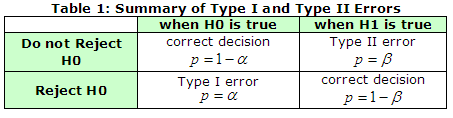
\includegraphics[width=0.7\linewidth]{images/typeIandIIerror}
\end{figure}






\subsection{Finite Population Correction Factor}

If the sample size is more than 5\% of the population size and the sampling is done without replacement, then a correction needs to be made to the standard error of the means.

In the following, N is the population size and n is the sample size. The adjustment is to multiply the standard error by the square root of the quotient of the difference between the population and sample sizes and one less than the population size.  

For the most part, we will be ignoring this in class







\end{document}

